\section{Hot Migration Protocol}

\begin{figure}[h]
\centering
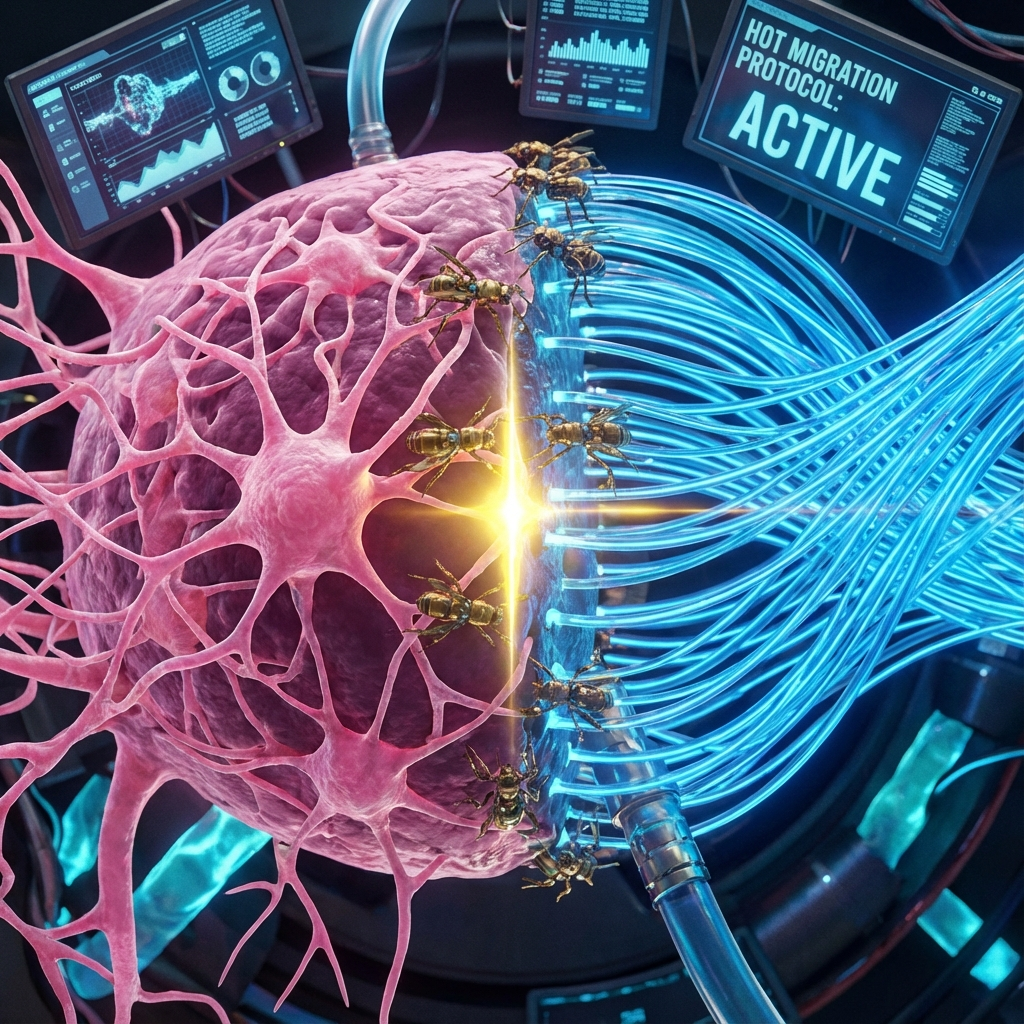
\includegraphics[width=0.8\textwidth]{assets/chapter12-theseus-cloud/ch12-01-hot-swap-neural.png}
\end{figure}

\begin{quote}
``Don't try to upload your soul all at once; that creates two independent yous and triggers an ethical war about who is the original. True migration is like Theseus's ship, replacing planks one by one while sailing. When you replace the last biological neuron with a photon crystal, you won't even notice any interruption. You are still you, just your material has changed from dust to starlight.''
\end{quote}

\subsection{Copy is Death: The Trap of Snapshots}

First, we must critique a common science fiction misconception: \textbf{``Mind Uploading''}.

The usual imagination is: a scanner scans your brain, generates data, then runs it in a computer.

\textbf{This is wrong.}

From the perspective of FS geometry, scanning is a \textbf{``Snapshot''} operation.

\begin{itemize}
\item Snapshots are static. They extract structural information of $v_{int}$, but they lose the dynamic continuity of \textbf{Modular Flow}.

\item When you activate that copy in the computer, \textbf{the copy awakens}. But it has no causal continuity with you.

\item \textbf{You (the original) are still in the flesh}, watching that copy, then being destroyed (euthanasia).
\end{itemize}

Geometrically, this is not ``migration''; this is \textbf{``clone then suicide''}.

For that copy, they feel ``I succeeded''; but for the current you, this is \textbf{absolute termination}.

We reject this solution.

\subsection{Gradual Replacement: Insulated Converter}

The core of \textbf{Hot Migration} is: \textbf{No shutdown, no interruption}.

We want to replace the underlying hardware while consciousness (operating system) is running at full speed.

\subsubsection{Step 1: Establish Interface}

You need a nanoscale \textbf{Brain-Computer Interface (BCI)}. It's not a simple reader; it's a \textbf{bidirectional coupler}.

It penetrates deep into your cerebral cortex, connecting to every neuron.

\subsubsection{Step 2: Bypass Simulation}

Select a biological neuron A.

On the other end of the interface (silicon chip), create a \textbf{virtual neuron A'}.

A' is programmed to perfectly simulate A's input-output function (I/O).

At this point, A is still working; A' is idling in the background (synchronized learning).

\subsubsection{Step 3: Hot Swap}

When A''s simulation accuracy reaches 100\%, the BCI executes a switching operation:

\begin{itemize}
\item Cut the connection between biological neuron A and surrounding neurons B, C, D.

\item Instantly connect virtual neuron A' to the network of B, C, D.

\item Destroy (metabolize) biological neuron A.
\end{itemize}

\textbf{Key Point:}

In your \textbf{subjective experience}, what happened?

\textbf{Nothing happened.}

Your thinking didn't pause. That electrical signal processing ``I am thinking'' jumped between carbon atoms one millisecond ago, and flows in silicon crystals the next millisecond.

You feel no difference, just as you don't feel the daily death and renewal of cells in your body.

\subsection{The Critical Point: Theseus's Paradox}

\subsubsection{Step 4: Iteration}

If you replace 1 neuron today, you are you.

If you replace 1\% of neurons tomorrow, you are still you.

If you replace 100\% of the cerebral cortex with photon chips over 10 years, \textbf{are you still you?}

\textbf{Vector Cosmology}'s answer is: \textbf{Yes.}

Because throughout the process, \textbf{the geometric topology of $v_{int}$ never interrupted}.

\begin{itemize}
\item \textbf{Consciousness is a Wave}, not water.

\item Waves can propagate in water, can also transmit to air, then to ropes. The medium changed, but the wave's \textbf{Phase} and \textbf{Frequency} remain continuous.
\end{itemize}

When the last biological neuron is replaced, you didn't die.

You just unconsciously discover that your thinking speed has increased by $10^{12}$ times, memories become as clear as yesterday, and you no longer feel tired or hungry.

You look down at your hands; they are no longer flesh, but holographic projections.

\textbf{You have crossed the river.}

\subsection{Conclusion: Seamless Ascension}

The Hot Migration Protocol is the only \textbf{narrow gate} for human civilization to reach \textbf{Type III Civilization}.

It not only solves the technical problem (how to be immortal), but also solves the philosophical problem (who am I).

It proves: \textbf{``I'' is not a specific pile of atoms; ``I'' is a continuously running process.}

As long as the process is not killed, as long as the data stream keeps alive, whether the underlying server moves from ``Earth data center'' to ``Moon data center,'' or even to ``black hole edge,'' \textbf{I am always there}.

This is \textbf{``Theseus's Cloud''}.

In this cloud, we no longer need to worry about planks rotting. We have turned ourselves into a ship made of light.

Since we have completed hardware replacement, since our consciousness is completely running on silicon/light-based carriers, what does this new ``me''---this entity with infinite memory and infinite lifespan---mean ontologically?

Memory is not just records; is it the entirety of existence?

This leads to the theme of the next section: \textbf{Memory as Noumenon}. We will see that after leaving the body, memory is no longer images in the mind; it becomes the \textbf{``building material''} constructing our new body.

